\pdfoutput=1
\documentclass[twocolumn]{aastex62}
%%\documentclass[]{emulateapj}

%Accepted/received/... %%

\received{xxx}
\revised{yyy}
\accepted{zzz}

%% Command to document which AAS Journal the manuscript was submitted to.
\submitjournal{AAS Journals}

%% Short title/authors

\shorttitle{LXUV History of TRAPPIST-1}
\shortauthors{Fleming et al.}

%% Begin document, title, packages %%
\usepackage{hyperref}
\usepackage{xspace}
\usepackage{graphicx}
\usepackage{amsmath}
\usepackage[caption=false]{subfig}

%% Custom commands
\def\mearth{{\rm\,M_\oplus}}
\def\rearth{{\rm\,R_\oplus}}
\def\msun{{\rm\,M_\odot}}
\def\rsun{{\rm\,R_\odot}}
\def\lsun{{\rm\,L_\odot}}
\def\gsim{~\rlap{$>$}{\lower 1.0ex\hbox{$\sim$}}}
\def\lsim{~\rlap{$<$}{\lower 1.0ex\hbox{$\sim$}}}

\newcommand{\xxx}[1]{{\textbf{#1}}}
\newcommand{\vplanet}[0]{\texttt{VPLanet}\xspace}
\newcommand{\emcee}[0]{\texttt{emcee}\xspace}
\newcommand{\approxposterior}[0]{\texttt{approxposterior}\xspace}
\newcommand{\eqtide}[0]{\texttt{EQTIDE}\xspace}
\newcommand{\stellar}[0]{\texttt{STELLAR}\xspace}
\newcommand{\kepler}[0]{\textit{Kepler}\xspace}
\newcommand{\jwst}[0]{\textit{JWST}\xspace}

%% Begin doc %%
\begin{document}

\title{On The XUV Luminosity Evolution of TRAPPIST-1}

%% AUTHORS %%

%%\correspondingauthor{David P. Fleming}
%%\email{dflemin3@uw.edu}

%%\author[0000-0001-9293-4043]{David P. Fleming}
\author{David P. Fleming}
\affil{Astronomy Department, University of Washington \\
Box 951580, Seattle, WA 98195}
\affil{NASA Astrobiology Institute - Virtual Planetary Laboratory Lead Team, USA}

\author{Rory Barnes}
\affiliation{Astronomy Department, University of Washington \\
Box 951580, Seattle, WA 98195}
\affil{NASA Astrobiology Institute - Virtual Planetary Laboratory Lead Team, USA}

\author{Jake VanderPlas}
\affiliation{Google \\
601 N 34th St, Seattle, WA 98103}

\author{Rodrigo Luger}
\affil{NASA Astrobiology Institute - Virtual Planetary Laboratory Lead Team, USA}
\affiliation{Center for Computational Astrophysics, Flatiron Institute \\
New York, NY 10010}

%% ABSTRACT %%

\begin{abstract}

Abstract.

- we constrain the stellar evolution and mass of TRAPPIST-1 using best priors and constraints currently available. we make our posterior distributions available for use with water loss simulations as the FXUV is a core input to such models, be it energy limited or recombination limited, maybe non-thermal escape models as well (look into that). our model and machine learning approach is all open source and documented on github, including a repo for the project itself
- TRAPPIST-1 conference stellar evolution stuff is 1st day, so email invited talks presenters and send them draft and thank them for their work which I use and cite in my own work - adam burgasser and jeff linsky
- 5 plots/tables: table of priors; corner plot; L, LXUV, R sampled from posteriors; \approxposterior comparison plot with distributions on top of each other 
- from Peacock+2018: "Late-type M stars remain UV active for much longer than their early M counterparts, typically with more variability in the FUV than the NUV (Miles Shkolnik 2017)."

\end{abstract}

%% Keywords %%

\keywords{}

%% Intro %%

\section{Introduction} \label{sec:intro}

-look at Rory's XRP for good references to mass-loss mechanisms

-\citet{Reiners2014} find that rotation period can determine Lx
\citet{Newton2017} find that LHalpha, an activity indicator saturates as low Prot/Ro with the cutoff occuring at a similar Ro to other inidicators like Lx

-For low-mass stars in the saturated phase, $L_{X}$ remains a constant fraction of $L_{bol}$ and is observed to cluster around $\log_{10}(L_X/L_{bol}) \approx -3$ \citep{Pizzolato2003,Wright2011,Wright2018}. 

"Although the dynamo processes that drive stellar activity and XUV emission in fully-convective stars have been shown to evolve qualitatively similar to solar-type stars \citep{Wright2016,Wright2018} ..."

- define XUV, what it is, and why it's important

-Introduction about stellar activity for late type stars, what it is like and how late type stars evolve, and finally why it matters for exoplanet habitability, e.g. the XUV flux is a critical parameter for atmospheric escape and water loss, other loss mechanisms scale as FXUV to some power, like energy-limited and recombination-limited escape. In the intro, I explain what saturated and unsaturated phases correspond to physically, and under what conditions they are expected to occur. Argue how this qualitative behavior is observed for both partially and fully-convective stars, e.g. FGK and M dwarfs.

-This study is critical and timely since people are modeling the hell out of TRAPPIST-1 and its planets and JWST proposals are going in to observe this system. My approach is generic and applicable to any systems with data and is relevant for LUVOIR where it can observe a statistically meaningful sample of planets, need \approxposterior for speed for constraints

-The saturation ratio shows tentative evidence of increasing with decreasing stellar mass \citep{Wright2011,Jackson2012}, consistent with the observation that later type low-mass stars are more active \citep[e.g.][]{West2008}. 

-"Stellar XUV flux cannot be reliably determined as it is heavily absorbed by the ISM
even for closest stars. However, XUV fluxes are required input parameters for the characterization
of photoionization and photodissociation which are crucial for modeling exoplanetary atmospheric
dynamics and escape (Ribas+2005; Airapetian+2017a; Garcia-Sage+2017; Johnstone+2018; 
Lammer 2018; Glocer+2018). This effort should be combined with empirical and semi-empirical
methods which reconstruct XUV fluxes using FUV/NUV and radiative transfer modeling efforts
(Linsky+2013; France +2016; Peacock+2018; Richey-Yowell+2019)."

-"stellar ionizing radiation including soft X-ray and Extreme
Ultraviolet, EUV (100 – 920 Å) later referred to as XUV"

-"It is also known
that the rotation velocity of a star is correlated with its magnetic activity specified by X-ray
flux (Güdel 2007)."

-"most of stellar XUV emission remains
hidden from us because most of the EUV flux longer that 40 nm is absorbed by interstellar
medium even from the closest stars."

-"The XUV stellar spectrum is crucial for understanding the
exoplanetary atmospheric evolution and its impact on habitable worlds as it drives and regulates
atmospheric heating, mass loss and chemistry on Earth-like planets, and thus is critical to the
long-term stability of terrestrial atmospheres."

-"The stellar XUV emission can be reconstructed using empirical and theoretical
approaches. Empirical reconstructions have already provided valuable insights on the level of
ionizing radiation from F, K, G and M dwarfs (Cuntz & Guinan 2016; France et al. 2016; 2018;
Loyd et al. 2016; Youngblood et al. 2016; 2017). "

- "Assuming N+/O+ ~ 1 during large
geomagnetic storms driven by flare and CME events, the total ion mass loss rate scales as" ion (O+, N+) escape rate scales linearly with FXUV

-"Lighter species, such as hydrogen, tend to escape more easily through thermal escape, but
strong XUV fluxes can also stimulate the loss of light and heavy ions through ionospheric
outflow and exospheric pick-up by stellar winds (Glocer et al. 2012; Airapetian et al. 2017a;
Kislyakova et al. 2014; Dong et. al. 2017; Lammer et al. 2008; 2018)."

-"Way et al. (2016) summarize possible scenarios of the
water evolution on early Venus. They note that the early water inventory was likely lost within
~100 Myrs of years after formation due to atmospheric escape driven by XUV flux from the
active young Sun (see also Chassefiere 1997 and Ramirez and Kaltenegger 2014)."

\section{Model} \label{sec:model}

We simulate TRAPPIST-1's evolution using the \stellar module in \vplanet \citep{Barnes2016,vplanet2018} that performs a bicubic interpolation over mass and age of the \citet{Baraffe2015} stellar evolution tracks. The \citet{Baraffe2015} models, also employed by both \citet{Burgasser2017} and \citet{vanGrootel2018} to constrain TRAPPIST-1's stellar properties, were computed for solar metallicity stars and hence are suitable for TRAPPIST-1 whose [Fe/H] is consistent with solar \citep{Gillon2016}, although \citet{Burgasser2017} argue TRAPPIST-1 has a slightly super-solar metallicity based on isochrone modeling.

The X-ray luminosity, L$_{X}$, evolution of fully convective stars follows the same broken power law model examined for partially-convective FGK stars \citep{Wright2016,Wright2018}. We assume TRAPPIST-1's L$_{XUV}$ evolution traces that of L$_{X}$ and simulate the $L_{XUV}$ evolution using the broken power law model of \citet{Pizzolato2003} and \citet{Ribas2005} implemented in \stellar as
\begin{align}
\label{eqn:lxuv}
\frac{L_\mathrm{XUV}}{L_\mathrm{bol}} = \left\{
				\begin{array}{lcr}
					f_\mathrm{sat} &\ & t \leq t_\mathrm{sat} \\
					f_\mathrm{sat}\left(\frac{t}{t_\mathrm{sat}}\right)^{-\beta_\mathrm{XUV}} &\ & t > t_\mathrm{sat}
				\end{array}
				\right.
\end{align}
where $f_{sat}$ is the constant ratio of stellar XUV to bolometric luminosity during the saturated phase, $t_{sat}$ is the duration of the saturated phase, and $\beta_{XUV}$ is the exponent that controls how steeply L$_{XUV}$ decays after saturation.

%% MCMC %%

\section{Markov Chain Monte Carlo} \label{sec:mcmc}

We use \texttt{emcee} \citep{ForemanMackey2013}, a Python implementation of the \citet{Goodman2010} affine-invariant Metropolis-Hastings Markov Chain Monte Carlo (MCMC) sampling algorithm, to infer posterior probability distributions for our model parameters. These parameters comprise the state vector
\begin{equation}
    \textbf{x} = \{m_{\star}, f_{sat}, t_{sat}, \mathrm{age}, \beta_{XUV}\},
\end{equation}
where $m_{\star}$ and age are the stellar mass and age, respectively, and the other parameters are defined by Eqn.~\ref{eqn:lxuv}.  MCMC sampling allows us to derive probability distributions for our model parameters that are conditioned on observations and our understanding on the underlying physics while accounting for correlations between parameters and their observational uncertainties.  

Note that our method to derive probabilistic constraints for TRAPPIST-1's stellar and XUV evolution is applicable to any low-mass star with measured $L_{bol}$ and $L_{XUV}$ for use with studies examining the water loss history of exoplanets or their evolving space weather environment (XXX cite). Additional constraints for individual systems, e.g. age estimates, improve both the accuracy and precision of the derived probabilistic constraints.  

\subsection{Priors} \label{sec:mcmc:priors}

With only two data points to condition our analysis, $L_{bol}$ and $L_{XUV}$, our prior probability distributions will strongly impact our results. We leverage observations of TRAPPIST-1 and late M dwarfs to assemble the best available empirical constraints to serve as priors for our MCMC analysis of TRAPPIST-1 and that are applicable to any fully-convective M dwarfs. We summarize our adopted distributions in Table~\ref{tab:priors}.

Following \citet{vanGrootel2018}, we rely on TRAPPIST-1's luminosity (here in our likelihood function, Eqn.~\ref{eqn:lnlike}) and age to constrain its mass and therefore adopt a flat prior of $m_{\star} \sim \mathcal{U}(0.07, 0.11)$. We use the empirical age constraint for TRAPPIST-1 derived by \citet{Burgasser2017}, age $\sim \mathcal{N}(7.6, 2.2^2)$ Gyr, as their thorough analysis considered both observations of TRAPPIST-1 and a host of empirical age indicators for ultracool dwarfs. 

We construct an empirical $f_{sat} = \log_{10}(L_{XUV}/L_{bol})$ distribution for late M dwarfs from the sample of fully-convective, saturated stars with observed $L_{X}$ from \citet{Wright2011}. For each star in the \citet{Wright2011} sample, we follow \citet{Wheatley2017} and estimate $L_{XUV}$ as a function of L$_{X}$ using Eqn.~(2) from \citet{Chadney2015}. We find that the distribution of $f_{sat}$ for fully-convective, saturated M dwarfs is well-approximated by a normal distribution, $f_{sat} \sim \mathcal{N}(-2.92, 0.26^2)$, and we adopt it as our prior. 

The duration of the saturated phase is estimated to be $t_{sat} \approx 100$ Myr for FGK stars \citep{Jackson2012}. Studies of stellar activity of late type stars as a function of stellar age, or its proxy, rotation period, indicate that the activity lifetime, and hence duration of the saturated phase, is likely longer for later-type stars \citep{Shkolnik2014,Wright2011,West2015,GonzalezAlvarez2019}, with fully-convective M dwarfs potentially remaining active for Gyrs, up to the ages of field stars \citep{West2008,Schneider2018}. TRAPPIST-1's high observed L$_{X}$ \citep{Wheatley2017}, short photometric rotation period \citep[3.3 d, ][]{Luger2017}, and low Rossby number \citep[Ro $\approx 0.01$, ][]{Roettenbacher2017,Wright2018} suggest that TRAPPIST-1 is still saturated today \citep{Pizzolato2003,Wright2011,Wright2018,Garraffo2017,GonzalezAlvarez2019}. Both \citet{Roettenbacher2017} and \citet{Morris2018} suggest that the photometrically-determined rotation period is inaccurate, with the latter study proposing that the 3.3 d period corresponds to a characteristic timescale for active regions on the stellar surface, but TRAPPIST-1's $v \sin i = 6$ km s$^{-1}$ \citep{Barnes2014} implies a rotation period of $\approx 1$ d for $i = 90^{\circ}$, providing evidence that TRAPPIST-1's rapid rotation is physical and consistent with saturation.  Given these constraints, we adopt a broad uniform $t_{sat}$ prior distribution over $0.1 - 12$ Gyr.

In the unsaturated phase, $L_{X}$, and hence $L_{XUV}$, fall off exponentially with powerlaw slope $\beta_{XUV}$ \citep{Ribas2005}. \citet{Jackson2012} find that $\beta_{XUV}$ does not vary significantly with stellar mass in their sample of FGK stars, and \citet{Wright2016} found that the X-ray evolution of fully-convective stars is qualitatively similar to that of partially-convective FGK stars. Therefore, we adopt the distribution derived from the \citet{Jackson2012} sample of late K dwarfs as our prior: $\beta_{XUV} \sim \mathcal{N}(-1.18, 0.31^2)$.

\begin{deluxetable}{lcc}
\tabletypesize{\small}
\tablecaption{Prior Distributions \label{tab:priors}}
\tablewidth{0pt}
\tablehead{
\colhead{Parameter [units]} & \colhead{Prior} & \colhead{Notes}
}
\startdata
$m_\star$ [$M_{\odot}$] & $\mathcal{U}(0.07, 0.11)$ & -- \\  
$f_{sat}$ & $\mathcal{N}(-2.92, 0.26^2)$ & \citet{Wright2011},  \\
 &  & \citet{Chadney2015}  \\
$t_{sat}$ [Gyr] & $\mathcal{U}(0.1, 12)$ & -- \\
age [Gyr] & $\mathcal{N}(7.6, 2.2^2)$ & \citet{Burgasser2017} \\
$\beta_{XUV}$ & $\mathcal{N}(-1.18, 0.31^2)$ & \citet{Jackson2012}
\enddata \vspace*{0.1in}
\end{deluxetable}

\subsection{Likelihood Function and Convergence}

We condition our analysis on the observed the bolometric luminosity, $L_{bol} = 5.22 \pm{0.19} \times 10^{-4} \ L_{\odot}$ \citep{vanGrootel2018} and XUV luminosity, $L_{XUV} = 3.9 \pm{0.5} \times 10^{-7} \ L_{\odot}$ \citep{Wheatley2017}. We computed $L_{XUV}$ by convolving the \citet{vanGrootel2018} $L_{bol}$ measurement and its uncertainty with the $L_{XUV}/L_{bol}$ constraints from \citet{Wheatley2017}.

For a given state vector \textbf{x}, we define our loglikelihood function as
\small
\begin{equation} \label{eqn:lnlike}
\begin{split}
    \ln \mathcal{L} \propto & -\frac{1}{2} \left[ \frac{(L_{bol} - L_{bol}(\textbf{x}))^2}{\sigma_{L_{bol}}^2} + \frac{(L_{XUV} - L_{XUV}(\textbf{x}))^2}{\sigma_{L_{XUV}}^2} \right] \\
    & + \ln \mathrm{Prior}(\textbf{x}) + C
\end{split}
\end{equation}
\normalsize
where $L_{bol}$, $L_{XUV}$ and $L_{bol}(\textbf{x})$, $L_{XUV}(\textbf{x})$ are the observed values and \vplanet outputs given \textbf{x}, respectively, $\sigma_{L_{bol}}$ and $\sigma_{L_{XUV}}$ are the observational uncertainties, $\ln \mathrm{Prior}(\textbf{x})$ is the prior probability, and $C$ is an arbitrary constant. 

With our likelihood function and priors specified, we run our MCMC analysis with 100 parallel chains for 10,000 iterations, initializing each chain by randomly sampling each element of \textbf{x} from their respective prior distributions. Each step of the MCMC chain, \vplanet takes \textbf{x} as input and simulates TRAPPIST-1's evolution up to its age, predicting $L_{bol}$ and $L_{XUV}$ to evaluate the likelihood function. We discard the first 500 iterations as burn-in and assess the convergence of our MCMC chains by computing the integrated autocorrelation length and acceptance fraction for each chain. We find a mean acceptance fraction of 0.45 and a minimum and mean number of iterations per integrated autocorrelation length of 75 and 110, respectively, indicating that our chains have likely converged.

%% Results %%

\section{Results} \label{sec:results}

In Fig.~\ref{fig:corner}, we display the posterior probability distributions for our model parameters derived by our MCMC analysis, adopting the median values of the marginal distributions as our best-fit solutions and derive the lower and upper uncertainties from the 16th and 84th percentiles, respectively. TRAPPIST-1 likely maintained a large $L_{XUV}$ throughout its lifetime, with our MCMC analysis uncovering strong correlations between the model parameters that control this evolution. We find TRAPPIST-1's $f_{sat} = -3.05^{+0.24}_{-.1}$ and $t_{sat} = 6.85^{+3.43}_{-3.15}$ Gyr, both deviating significantly from their priors and consistent with observed $L_{XUV}/L_{bol}$ and long activity lifetimes of late M dwarfs (XXX citations). The long upper-tail in the marginalized $f_{sat}$ distribution arises from the combination of the degeneracy between $f_{sat}$ and $t_{sat}$ and from our strong empirical $f_{sat}$ prior that disfavors $f_{sat} \gsim -2.7$. Large $f_{sat}$ require short $t_{sat}$, and hence earlier powerlaw $L_{XUV}$ decay during the unsaturated phase, to match TRAPPIST-1's observed $L_{XUV}$, and vice-versa. From the joint posterior distribution, we infer that there is a $42.6\%$ chance that TRAPPIST-1 is still in the saturated phase today, i.e. P$(t_{sat} \geq \mathrm{ age } | \mathrm{data}) \approx 0.426$. Our analysis strongly disfavors short saturation timescales, with only a $0.4\%$ chance that $t_{sat} \leq 1$ Gyr, the saturation timescale adopted by \citet{Luger2015} in their analysis of water loss from exoplanets orbiting in the habitable zone of late M dwarfs. These constraints imply that TRAPPIST-1 has likely maintained a high XUV luminosity throughout its lifetime, potentially driving extreme water loss from its planets (XXX citation).

\begin{figure*}[t]
\centering
	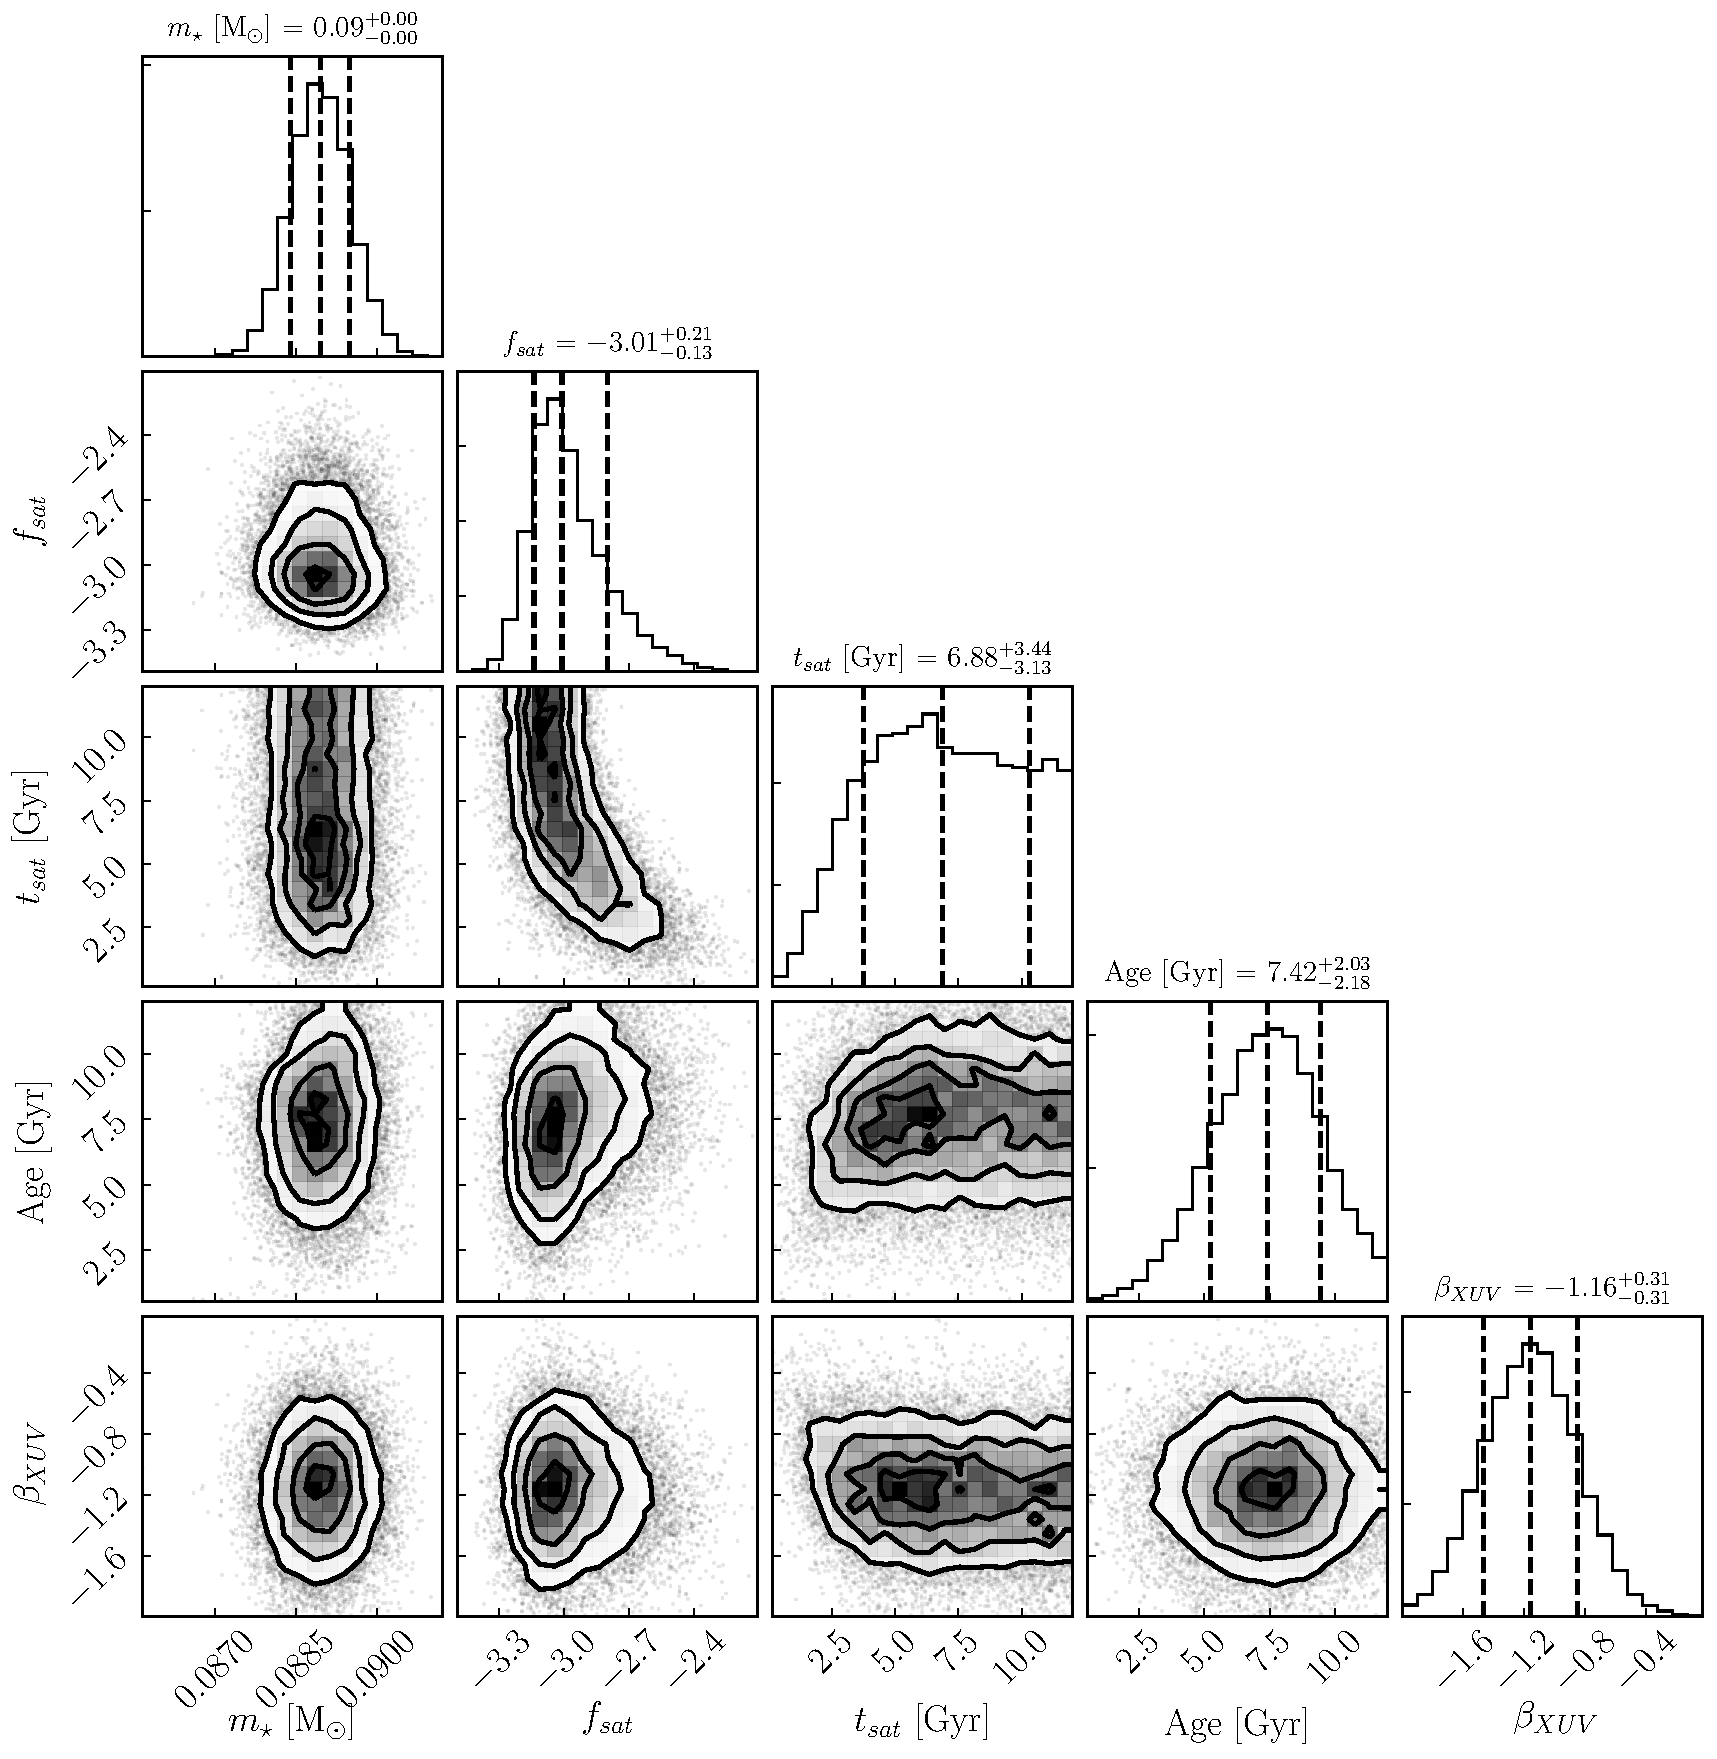
\includegraphics[width=0.75\textwidth]{../Analysis/Corner/trappist1Corner.pdf}
   \caption{Joint and marginal posterior probability distributions for the TRAPPIST-1 stellar parameters (XXX state vector eqn) made using \texttt{corner} \citep{ForemanMackey2016}. The black vertical dashed lines on the marginalized distributions indicate the median values and lower and upper uncertainties from the 16th and 84th percentiles, respectively. From the posterior, we infer that there is a $42.6\%$ chance that TRAPPIST-1 is still in the saturated phase today, potentially driving significant water loss and atmospheric escape from its planets.}%
    \label{fig:corner}%
\end{figure*}

We constrain TRAPPIST-1's mass to $m_{\star} = 0.089^{+0.0006}_{-0.0006}$ M$_{\odot}$, identical to the \citet{vanGrootel2018} constraint. Our marginalized age and $\beta_{XUV}$ posterior distributions reflect their prior distributions as for the former, $L_{bol}$ is not sufficient to further constraint TRAPPIST-1's age beyond our adopted prior since the luminosities of M dwarfs do not significantly change on the main sequence \citep{Baraffe2015}. We do not further constrain $\beta_{XUV}$ because our model prefers to exploit the degeneracy between $f_{sat}$ and $t_{sat}$ to match TRAPPIST-1's observed $L_{XUV}$, instead of varying the slope of the $L_{XUV}$ decay during the unsaturated phase, likely because TRAPPIST-1 is still saturated, rendering $\beta_{XUV}$ unnecessary to model its $L_{XUV}$ evolution. Age and $\beta_{XUV}$ weakly correlate with $f_{sat}$, both requiring a narrow spread of $f_{sat} \approx -3.05$ for young ages and steeper $\beta_{XUV}$. $\beta_{XUV}$ and $t_{sat}$ are uncorrelated, except at short $t_{sat}$ where steep $\beta_{XUV}$ are disfavored.

\subsection{TRAPPIST-1's Evolutionary History}

Here we consider plausible stellar evolutionary histories for TRAPPIST-1, conditioned on observations, by evolving 100 draws from the posterior distribution using \vplanet. We plot the evolution of TRAPPIST-1's $L_{bol}$, $L_{XUV}$, and radius in Fig.~\ref{fig:evol} and compare our models to the measured values. 

\begin{figure*}[t]
	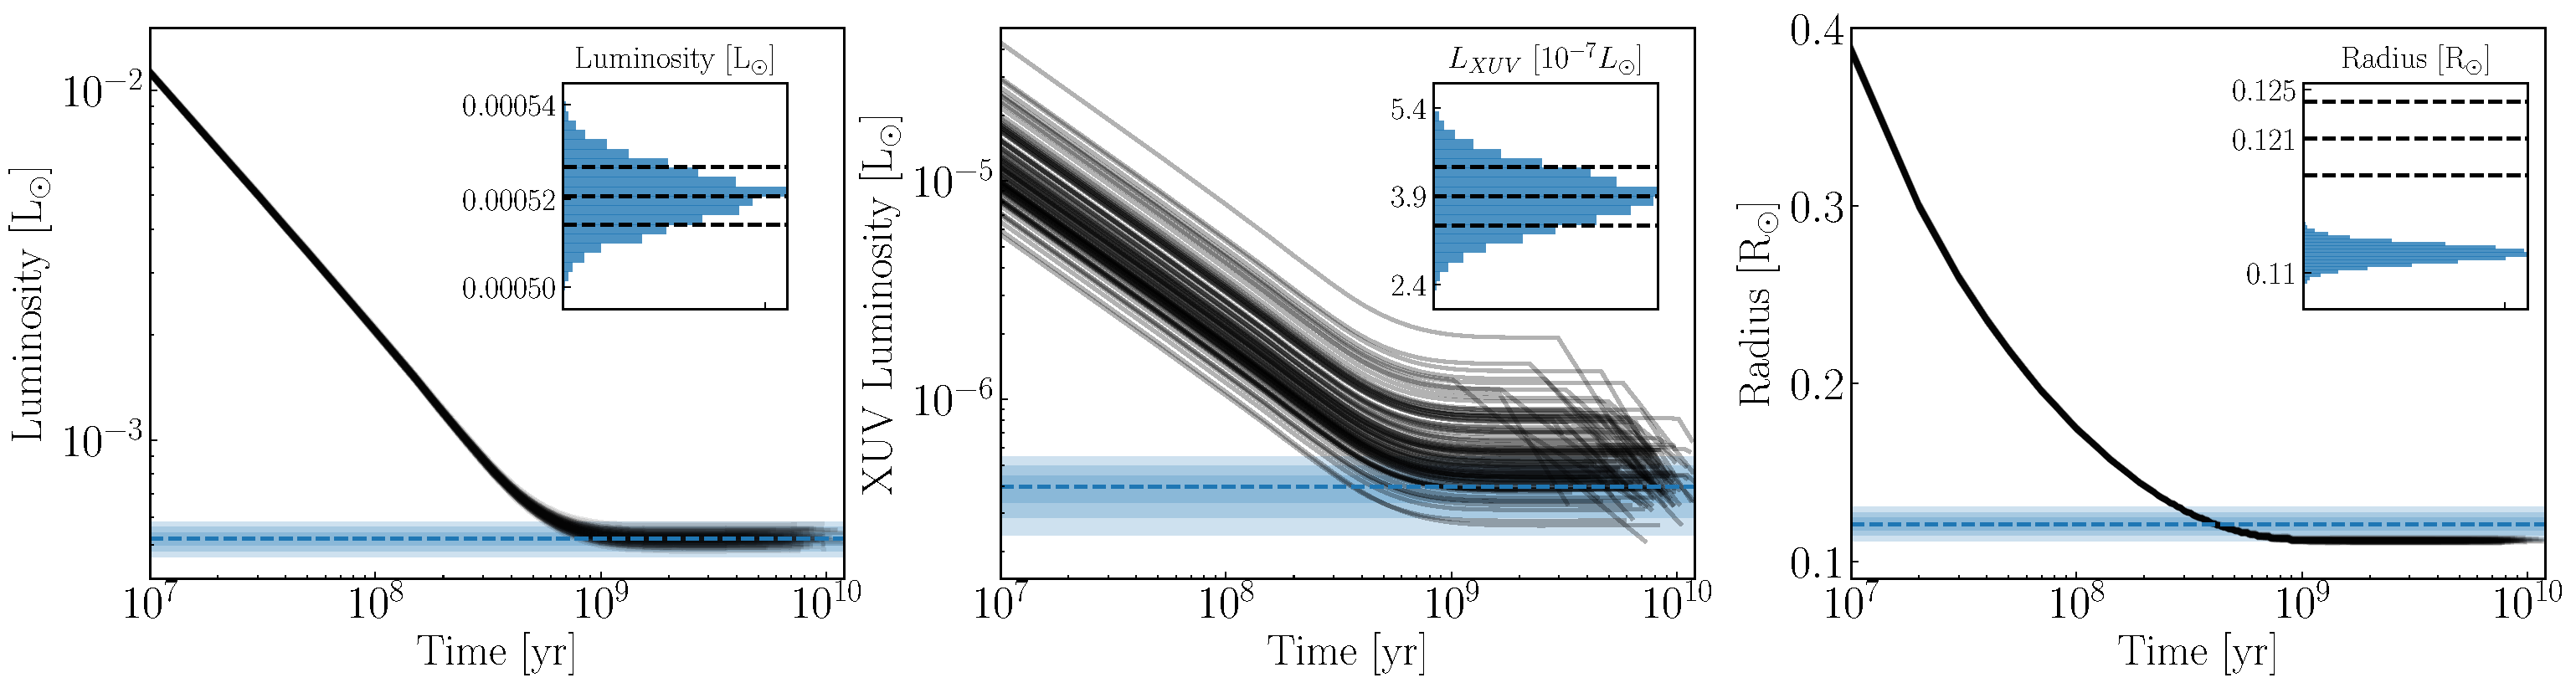
\includegraphics[width=\textwidth]{../Analysis/Evol/trappist1Evol.pdf}
   \caption{Plausible evolutionary histories of TRAPPIST-1's bolometric luminosity (left), XUV luminosity (center), and radius (right) using 100 samples drawn from the posterior distribution and simulated with \vplanet. In each panel, the blue shaded regions display the 1, 2, and 3 $\sigma$ the observational uncertainties. The insets display the marginalized distributions (black) evaluated at the age of the system, with the blue dashed lines indicating the observed value and +/- 1 $\sigma$ uncertainty. The radius and bolometric luminosity constraints are adopted from \citet{vanGrootel2018}, and the L$_{XUV}$ constraint is taken from \citet{Wheatley2017}.}%
    \label{fig:evol}%
\end{figure*}

Since TRAPPIST-1 could still be saturated today, its planetary system has likely experienced a persistent extreme XUV environment, potentially driving massive water loss \citep[][;Fleming et al., in prep]{Luger2015,Bolmont2017,Bourrier2017}. For example, from our posterior distributions, we infer that TRAPPIST-1b, if its remained near its current semi-major axis after migration halted once its natal gaseous disk dissipated \citep{Luger2017}, likely received from $XXX \times F_{XUV,\ocross}$ over TRAPPIST-1's ${\sim}1$ Gyr pre-main sequence lifetime. TRAPPIST-1's $L_{XUV}$ evolution mainly tracks $L_{bol}$, with both decreasing by a factor of ${\sim}40$ along the pre-main sequence before stabilizing on the main sequence, with ${\sim}60\%$ of $L_{XUV}$ evolutions entering the unsaturated powerlaw decay at late times near the age of the system. 

TRAPPIST-1's radius likely shrank by roughly a factor of 4 along the pre-main sequence, with our posterior present-day radius $R_{\star} = 0.11 \pm{0.0008} \ R_{\odot}$. Our posterior radius is ${\sim} 8\%$ smaller than the \citet{vanGrootel2018} constraint, $R_{\star} = 0.121 \pm {0.003} \ R_{\odot}$, that was computed from their inferred mass and TRAPPIST-1's density \citep{Delrez2018}. This difference arises from the likely underprediction of TRAPPIST-1's radius by the \citet{Baraffe2015} models, consistent with stellar evolution models often underestimating the radii of late M dwarfs \citep{Reid2005,Spada2013,Jackson2019}, and suggests that TRAPPIST-1 might have super-solar metallicity \citep{Burgasser2017,vanGrootel2018}. If we instead follow \citet{vanGrootel2018} and compute the radius from our marginalized stellar mass posterior distribution and the \citet{Delrez2018} density constraint, we obtain $R_{\star} = 0.12 \pm{0.002} \ R_{\odot}$, in agreement with the \citet{vanGrootel2018} constraint.

%% approxposterior %%

\section{\approxposterior} \label{sec:approx}

-cite meadows 2018, andrew and jake's papers, ask them for other good citations
-wonderlick, morley, jake's paper for how far our we could observe

This analysis could be applied to the ${\sim}XXX$ stars within $XXX$ pc to characterize the XUV flux histories of any known or putative exoplanets they may host, given sufficient observational constraints for each star, e.g. bolometric and XUV luminosities. This sample of stars includes FGKM dwarfs, spectral types for which good priors to constrain the XUV evolution exist, and is of particular interest as all are close enough for future space missions missions, e.g. \jwst (XXX cite), to potentially detect and characterize the atmospheres of any terrestrial exoplanets they may host. The TESS (XXX cite) mission is currently observing the nearby brightest stars to detect transiting planets, increasing the number of known near-by potentially-habitable planets. Characterizing their water loss environments is important. (XXX jotted ideas down in this paragram, edit into coherent argument)  The MCMC presented in this work required 3,700 core hours on the University of Washington Hyak supercomputer system. Assuming similar convergence properties, repeating this analysis for the the ${\sim}XXX$ stars within $XXX$ pc would require $XXX$ core-hours, a non-trivial computational expense. Here, we apply \approxposterior, a Python machine learning package for the approximate inference of Bayesian posterior distributions, to our inference of TRAPPIST-1's XUV evolution to derive accurate approximations to the true MCMC-derived posteriors using only $XXX$ simulations and $XXX$ core hours, a fraction of the amounts used in our MCMC analysis.

Collaborator Fleming led the development of the \approxposterior package that employs machine learning to rapidly infer accurate approximations to the true posterior distributions of model parameters for Bayesian inference \cite[][Fleming et al., in prep]{FlemingVanDerPlas18}. This publicly available code can converge over 1000x faster than standard Markov Chain Monte Carlo (MCMC) samplers (e.g., \emcee \citealp{ForemanMackey13}), see $\S$~II and \cite{FlemingBarnes19}. In conjunction with \vplanet, these packages will enable the team to identify, quantify and understand the evolutionary trajectories of exoplanets and probablistically probe model degeneracies based on observational data and uncertainties.

We will use the statistical analysis code \approxposterior to compute Bayesian posterior distributions for model parameters, given observational constraints on a system, while minimizing the number of forward model (\vplanet) evaluations. This package is a Python implementation of the Bayesian Active Learning for Posterior Estimation method of \cite{Kandasamy15}, an adaptive learning Gaussian process (GP) approximation for Bayesian inference with expensive likelihood functions. This algorithm computes approximate posterior probability distributions by training a GP surrogate for the likelihood evaluation used for MCMC. The algorithm then leverages the inherent uncertainty in the GP's predictions to identify regions in parameter space that require forward model evaluations. By re-training the GP to maximize its predictive ability, the number of forward model evaluations is minimized. As an example, Fig.~XXX compares the results between \emcee and \approxposterior in evaluating the stellar parameters of TRAPPIST-1 conditioned on the observations of \citet{Grimm18} and \citet{Wheatley17}. The results are very similar, but the \approxposterior result required just 0.05\% as much CPU time.


%% Discussion %%

\section{Discussion and Conclusions} \label{sec:discussion}

Discuss, and then conclude.

Our results suggest that the atmospheric erosion of the TRAPPIST-1 planets could be on-going. Either a significant initial volatile mass fraction (XXX) or continual atmospheric replenishment via outgassing (XXX), perhaps driven by tidal interactions (XXX), are required to explain the TRAPPIST-1 planet's observed low densities \citep{Grimm2018}

The methods presented in this work can be applied to any other M dwarf with observed $L_{bol}$, $L_{XUV}$, and preferably age. Other works who are interested in constraining the water loss history of potentially-habitable exoplanets should build probabilistic models for the stellar evolution.

%% ACKNOWLEDGEMENTS %%
\acknowledgments
This work was facilitated though the use of advanced computational, storage, and networking infrastructure provided by the Hyak supercomputer system and funded by the Student Technology Fund at the University of Washington. DPF was supported by NASA Headquarters under the NASA Earth and Space Science Fellowship Program - Grant 80NSSC17K0482.  RB acknowledges support from the NASA Astrobiology Institute's Virtual Planetary Laboratory under Cooperative Agreement number NNA13AA93A.

%% SOFTWARE %%
\software{\approxposterior: \citet{FlemingVanderPlas2018}, \texttt{corner}: \citet{ForemanMackey2016}, \texttt{emcee}: \citet{ForemanMackey2013}, \texttt{matplotlib}: \citet{Hunter2007}, \texttt{numpy}: \citet{vanderWalt2011}, \vplanet: \citet{Barnes2016,vplanet2018}}, 

%% BIBLIOGRAPHY %%

\bibliography{trappist}

% End of file
\end{document}